\documentclass[../main.tex]{subfiles}

\begin{document}
Nella sezione precedente si \`e costruito il modello poi implementato tramite una libreria C++ reperibile, con relativa documentazione, sulla repository \url{https://github.com/Grufoony/TrafficFlowDynamicsModel}.
Tale modello dipende da diversi parametri di controllo, variando i quali \`e di fatto possibile ottenere risultati estremamente diversi tra di loro, permettendo lo svolgimento di pi\`u analisi.
In particolare, si andr\`a ora a effettuate tre tipologie di studi dove la rete viene caricata in modo omogeneo (inserendo contemporaneamente lo stesso numero di veicoli su tutte le strade):
\begin{itemize}
    \item \emph{carico costante}, ove il reticolo viene sottoposto ad un carico costante per un certo lasso di tempo;
    \item \emph{carico piccato}, in cui il reticolo viene sovraccaricato nei primi istanti, in modo tale da creare una congestione. Successivamente la rete viene lasciata svuotare per studiarne il comportamento;
    \item \emph{carico periodico}, dove il reticolo viene caricato nel tempo con un andamento sinusoidale, volto a rappresentare (grossolanamente) le diverse fasi di carico a cui una normale rete stradale \`e soggetta nell'arco di una giornata.
\end{itemize}
Il carico omogeneo non permette l'analisi del ruolo dei nodi sorgente i quali, salvo nei casi in cui i veicoli vengono reimmessi nella rete, perdono la loro funzione.
Questa scelta \`e stata effettuata in quanto lo studio \`e focalizzato sulle congestioni, fenomeni che sono difficilmente realizzabili con poche sorgenti e, nel caso, richiederebbero scale temporali non trascurabili rispetto alle scale temporali delle congestioni stesse.
Anche da un punto di vista pratico risulta pi\`u realistico supporre che i veicoli si immettano omogeneamente sulle strade (ipotizzando zone residenziali) e tendano a muovere verso alcuni punti attrattori, che possono essere supermercati, centri sportivi, ecc.\\
Una quarta e ultima analisi riguarda infine lo studio dei tempi di percorrenza, il cui scopo \`e di verificare gli andamenti previsti dalla teoria e in precedenza riportati in Fig. \ref{fig:frequency_distributions}.
Di questa, sono inoltre riportati in Appendice \ref{appendix:visual} delle rappresentazioni della rete stradale per favorire la visualizzazione dei fenomeni.


Si consideri ora un network composto da 120 nodi disposti in un reticolo 10x12.
\begin{figure}
    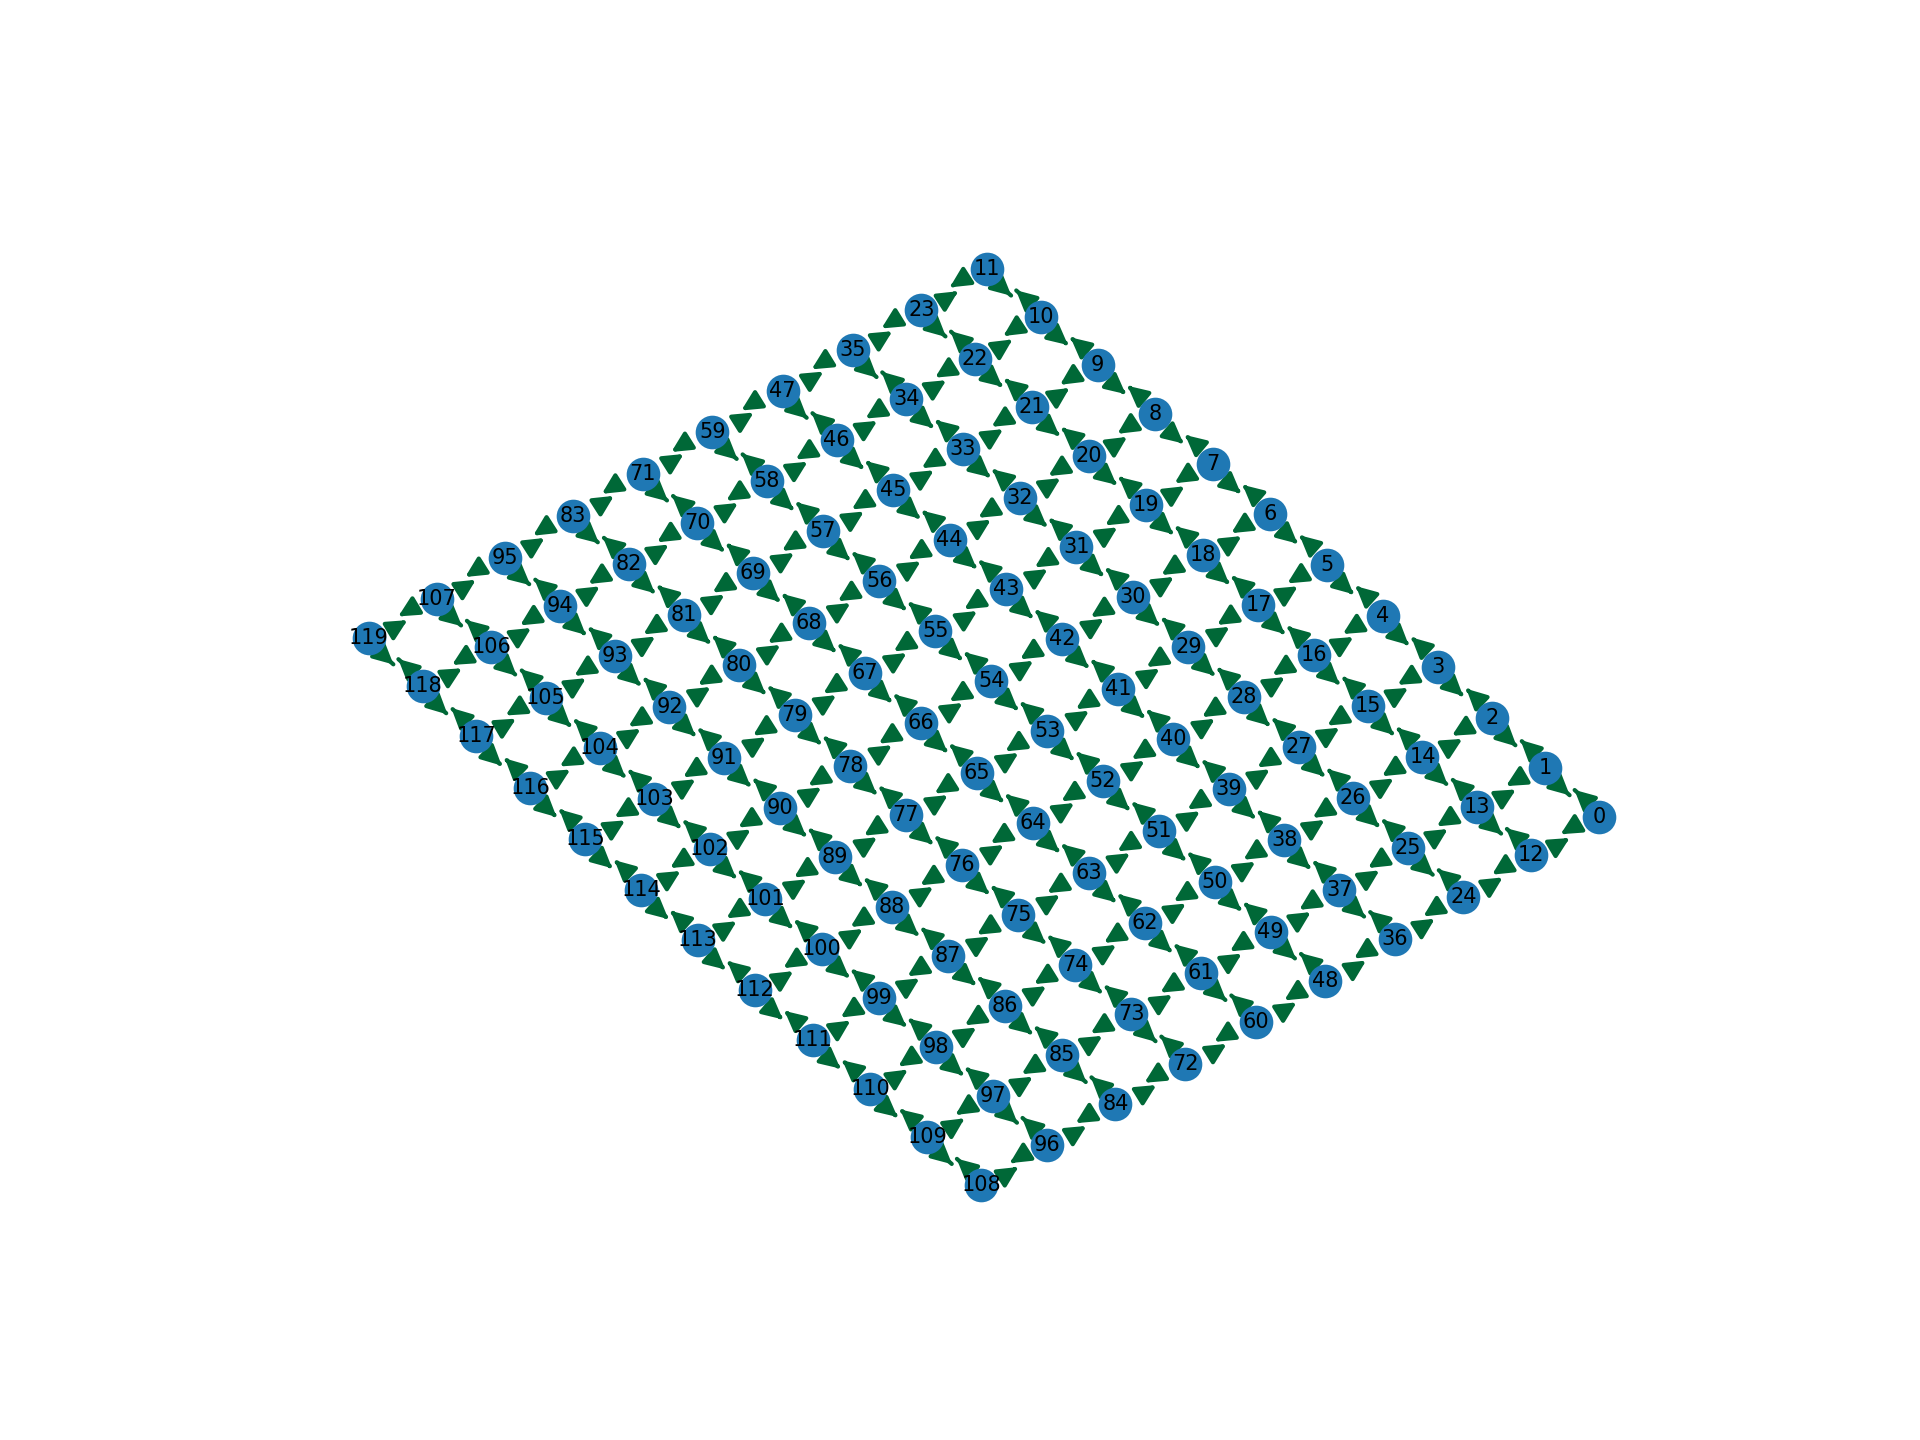
\includegraphics[scale=0.25, trim={2cm 5cm 10cm 5cm},clip]{./data/img/network.png}
    \caption[Network omogeneo]{\emph{Network omogeneo.}}
    \label{fig:network_homo}
\end{figure}
Su questo, si definiscano 16 differenti classi di veicoli, le cui sorgenti sono i nodi 1, 4, 7, 10 e le cui destinazioni sono i nodi 109, 112, 115, 118.
Risulta evidente dalla Fig. \ref{fig:network_homo} come i veicoli scorrano da un lato all'altro del reticolo.
Ogni strada ha lunghezza e velocit\`a massima fissate a 500 m e 50 km/h, rispettivamente.
Si pongano ora la lunghezza media di un veicolo pari a 8 m, la velocit\`a minima su una strada pari a $\frac{1}{4}$ della velocit\`a massima e una probabilit\`a di errore dell'8\%.

\section{Carico costante}
Si vuole, come prima cosa, sottoporre il sistema ad un carico costante: in questo modo si dovrebbe evitare la formazione di congestioni, mantenendo la capacit\`a di trasporto della rete stessa.
Il sistema viene quindi sottoposto ad un carico costante di 250 veicoli immessi ogni 60 s, fino a un tempo di 3.33 h, per un tempo totale di 4.15 h, lasciandoli liberi di uscire dalla rete una volta giunti a destinazione.
Ci si aspetta cos\`i una crescita iniziale della densit\`a media, la quale si mantiene costante fintantoch\'e nuovi veicoli vengono immessi nel sistema.
L'obiettivo \`e, infatti, mantenere complessivamente invariato il numero totale di veicoli presenti sulla rete, a meno di fluttuazioni.
\begin{figure}[H]
    \centering
    \begin{tikzpicture}
    \begin{axis}[
    grid = both,
    major grid style = {lightgray},
    minor grid style = {lightgray!25},
    width = 0.75\textwidth,
    height = 0.5\textwidth,
    ylabel near ticks,
    xlabel near ticks,
    xlabel = {Tempo (h)},
    ylabel = {Densit\`a media (veh/km)},]
    \addplot[
    mark size=0.69,
    draw=black,
    mark=o] file {./data/constant_homo/k-t.dat};
    \end{axis}
    \end{tikzpicture}
    \caption[Densit\`a media per un reticolo omogeneo con carico costante]{\emph{Densit\`a media per un reticolo omogeneo con carico costante.}}
    \label{fig:density_constant_homo}
\end{figure}
In Fig. \ref{fig:density_constant_homo} si pu\`o notare l'innalzamento iniziale, fino a circa 1.5 h, poi un regime pressoch\'e costante fino a 3.3 h, seguito da una rapida discesa.
Nell'arco temporale in cui la densit\`a \`e stabile ci si aspetta un regime di traffico completamente libero.
L'ipotesi \`e verificata in Fig. \ref{fig:nStreet_density_constant_homo} dove, graficando il numero di strade in funzione della densit\`a a 2 h, si pu\`o notare come la quasi totalit\`a di esse abbia densit\`a minima.
\begin{figure}[H]
    \centering
    \begin{tikzpicture}
    \begin{axis}[ybar interval,
    every tick label/.append style={font=\tiny},
    area style,
    width = 0.75\textwidth,
    height = 0.50\textwidth,
    xlabel = {$\frac{\rho}{\rho_{max}}$},
    ylabel = {Frequenza},]
    \addplot+[
    ybar interval,
    mark=no,
    line width = 1.25pt
    ] plot file {./data/constant_homo/7200_den.dat};
    \end{axis}
    \end{tikzpicture}
    \caption[Distribuzione delle strade non congestionate per un reticolo omogeneo.]{\emph{Distribuzione delle strade non congestionate per un reticolo omogeneo.}}
    \label{fig:nStreet_density_constant_homo}
\end{figure}
Non formandosi nessuna congestione ci si aspetta che il sistema si svuoti allo stesso modo in cui si \`e riempito.
In Fig. \ref{fig:hysteresys_constant_homo} \`e graficata la dipendenza tra i valori medi del flusso e della densit\`a.
In particolare, si nota come il grafico sia effettivamente una retta, il che implica che la curva di scarico sia sovrapposta a quella di carico.
\begin{figure}[H]
    \centering
    \begin{tikzpicture}[scale=0.75]
        \begin{axis}[
        grid = both,
        major grid style = {lightgray},
        minor grid style = {lightgray!25},
        width = 0.75\textwidth,
        height = 0.5\textwidth,
        ylabel near ticks,
        xlabel near ticks,
        xlabel = {Densità (veh/km)},
        ylabel = {Flusso (veh/h)},]
        \addplot[
        mark size=0.69,
        draw=black,
        mark=o] file {./data/constant_homo/q-k.dat};
        \end{axis}
    \end{tikzpicture}
    \caption[Diagramma flusso/densit\`a medi per un reticolo omogeneo sottoposto ad un carico costante.]{\emph{Diagramma flusso/densit\`a medi per un reticolo omogeneo sottoposto ad un carico costante.}}
    \label{fig:hysteresys_constant_homo}
\end{figure}

\section{Carico piccato}
Si inserisca ora nel sistema un totale di 25000 veicoli, suddivisi in 2500 veicoli ogni 50 s, consentendone la fuoriuscita dal reticolo solo dopo 67 min, in modo tale da lasciare al sistema tempo per giungere ad uno stato di equilibrio.
Si osserva cos\`i in Fig. \ref{fig:peaked_homo} un picco iniziale della densit\`a media (sovraccarico del sistema) e come questa rimanga stabile fino a circa 1 h da inizio simulazione, poi inizi a diminuire.
\begin{figure}[H]
    \centering
    \begin{tikzpicture}[scale=0.75]
    \begin{axis}[
    grid = both,
    major grid style = {lightgray},
    minor grid style = {lightgray!25},
    width = 0.75\textwidth,
    height = 0.5\textwidth,
    ylabel near ticks,
    xlabel near ticks,
    xlabel = {Tempo (h)},
    ylabel = {Densit\`a media (veh/km)},]
    \addplot[
    mark size=0.69,
    draw=black,
    mark=o] file {./data/peaked_homo/k-t.dat};
    \end{axis}
    \end{tikzpicture}
    \begin{tikzpicture}[scale=0.75]
        \begin{axis}[
        grid = both,
        major grid style = {lightgray},
        minor grid style = {lightgray!25},
        width = 0.75\textwidth,
        height = 0.5\textwidth,
        ylabel near ticks,
        xlabel near ticks,
        xlabel = {Tempo (h)},
        ylabel = {Flusso medio (veh/h)},]
        \addplot[
        mark size=0.69,
        draw=black,
        mark=o] file {./data/peaked_homo/q-t.dat};
        \end{axis}
        \end{tikzpicture}
    \caption[Densit\`a media per un reticolo omogeneo sovraccaricato]{\emph{Densit\`a media per un reticolo omogeneo sovraccaricato.}}
    \label{fig:peaked_homo}
\end{figure}
Una volta stabilizzato il sistema ci si aspetta che la distribuzione di veicoli nelle strade non resti omogenea nel tempo: gli agenti presenti sul sistema tenderanno ad occupare le strade costituenti i loro \emph{best path} e a lasciare vuote quelle pi\`u lontane da essi.
\begin{figure}[H]
    \centering
    \begin{tikzpicture}
    \begin{axis}[ybar interval,
    every tick label/.append style={font=\tiny},
    area style,
    width = 0.75\textwidth,
    height = 0.50\textwidth,
    xlabel = {Densit\`a (veh/km)},
    ylabel = {Frequenza},]
    \addplot+[
    ybar interval,
    mark=no,
    line width = 1.25pt
    ] plot file {./data/peaked_homo/5800_den.dat};
    \end{axis}
    \end{tikzpicture}
    \caption[Distribuzione delle strade congestionate per un reticolo omogeneo.]{\emph{Distribuzione delle strade congestionate per un reticolo omogeneo.}}
    \label{fig:nStreet_density_peaked_homo}
\end{figure}
In Fig. \ref{fig:nStreet_density_peaked_homo} \`e visibile il diagramma caratteristico della congestione, in cui sono presenti, come atteso, un gran numero di strade vuote e altrettante sature.
In questo istante di tempo, pari a 1.61 h da inizio simulazione, ci si aspetta dunque che i diagrammi fondamentali siano confrontabili con quelli in Fig. \ref{fig:greenshield}: questa ipotesi \`e confermata dalla Fig. \ref{fig:DMF_peaked_homo}.
\begin{figure}[H]
    \begin{tikzpicture}[scale=0.6]
    \begin{axis}[
    grid = both,
    major grid style = {lightgray},
    minor grid style = {lightgray!25},
    width = 0.75\textwidth,
    height = 0.5\textwidth,
    ylabel near ticks,
    xlabel near ticks,
    xlabel = {Flusso (veh/h)},
    ylabel = {Velocit\`a media (km/h)},]
    \addplot[
    mark size=0.69,
    draw=black,
    only marks] file {./data/peaked_homo/5800_u-q.dat};
    \end{axis}
    \end{tikzpicture}\hfill
    \begin{tikzpicture}[scale=0.6]
        \begin{axis}[
        grid = both,
        major grid style = {lightgray},
        minor grid style = {lightgray!25},
        width = 0.75\textwidth,
        height = 0.5\textwidth,
        ylabel near ticks,
        xlabel near ticks,
        xlabel = {Densità (veh/km)},
        ylabel = {Flusso (veh/h)},]
        \addplot[
        mark size=0.69,
        draw=black,
        only marks] file {./data/peaked_homo/5800_q-k.dat};
        \end{axis}
    \end{tikzpicture}
    \centering
    \begin{tikzpicture}[scale=0.6]
    \begin{axis}[
    grid = both,
    major grid style = {lightgray},
    minor grid style = {lightgray!25},
    width = 0.75\textwidth,
    height = 0.5\textwidth,
    ylabel near ticks,
    xlabel near ticks,
    xlabel = {Densit\`a (veh/km)},
    ylabel = {Velocit\`a media (km/h)},]
    \addplot[
    mark size=0.69,
    draw=black,
    only marks] file {./data/peaked_homo/5800_u-k.dat};
    \end{axis}
    \end{tikzpicture}
    \caption[DFM per una congestione]{\emph{Diagrammi fondamentali macroscopici di una congestione in un reticolo omogeneo.}}
    \label{fig:DMF_peaked_homo}
\end{figure}
Secondo la teoria dei flussi di traffico, un sistema congestionato tende a risolvere la congestione in modo differente da come questa si \`e formata e questo fenomeno causa la formazione di un ciclo di isteresi.
Lo scarico del sistema avviene gradualmente e prevede un ritorno alla stabilit\`a lungo una traiettoria differente rispetto alla fase di carico: tale differenza \`e visibile in Fig. \ref{fig:hysteresys_peaked_homo}.
\begin{figure}[H]
    \begin{tikzpicture}[scale=0.6]
        \begin{axis}[
        grid = both,
        major grid style = {lightgray},
        minor grid style = {lightgray!25},
        width = 0.75\textwidth,
        height = 0.5\textwidth,
        ylabel near ticks,
        xlabel near ticks,
        xlabel = {Densità (veh/km)},
        ylabel = {Flusso (veh/h)},]
        \addplot[
        mark size=0.69,
        draw=black,
        mark=o] file {./data/peaked_homo/q-k.dat};
        \end{axis}
    \end{tikzpicture}\hfill
    \begin{tikzpicture}[scale=0.6]
    \begin{axis}[
    grid = both,
    major grid style = {lightgray},
    minor grid style = {lightgray!25},
    width = 0.75\textwidth,
    height = 0.5\textwidth,
    ylabel near ticks,
    xlabel near ticks,
    xlabel = {Densit\`a (veh/km)},
    ylabel = {Velocit\`a media (km/h)},]
    \addplot[
    mark size=0.69,
    draw=black,
    mark=o] file {./data/peaked_homo/u-k.dat};
    \end{axis}
    \end{tikzpicture}
    \caption[Isteresi per un reticolo omogeneo sovraccaricato]{\emph{Ciclo di isteresi per un reticolo omogeneo sovraccaricato.}}
    \label{fig:hysteresys_peaked_homo}
\end{figure}
Si pu\`o notare come sia il flusso che la densit\`a crescano fino a un punto critico nel quale si ha un calo drastico del flusso stesso dovuto all'eccessiva presenza di veicoli sulle strade.
Il sistema risulta quindi congestionato e perde la capacit\`a di trasporto.
In particolare, il massimo del flusso si ha durante la fase di carico mentre, alla fine della stessa, il sovraccarico ha gi\`a apportato modifiche al sistema, riducendone il flusso medio (cfr. Fig. \ref{fig:peaked_homo}).
Inoltre, il flusso medio del sistema tende a rimanere stabile a ridosso della congestione, a differenza della densit\`a media che risulta gi\`a in diminuzione grazie alla fuoriuscita dei primi veicoli dalla rete.

\section{Carico periodico}
Si vuole ora sottoporre il sistema ad un carico realistico, quindi variabile nell'arco di una giornata.
Per semplicit\`a si decide di trascurare il carico notturno, in quanto nella maggior parte dei casi lascia il sistema in uno stato di traffico completamente libero.
Durante il giorno, invece, si assuma una variazione periodica con diversi picchi: il primo al mattino verso le ore 9:00, seguito da una lieve discesa, il secondo verso le 13:00, un po' meno marcato, e il terzo al rientro serale, alle 17:00.
Assumendo come orario di inizio simulazione le 5:45 del mattino, si immettano veicoli uniformemente nel sistema secondo la seguente funzione:
\begin{equation}
    \Delta n(t) = A \left\lvert \sin\left(\frac{2\pi}{T}t\right) \right\rvert 
\end{equation}
con $A = 2200$ veh e $T = 32400$ s.
In questo caso, non vi \`e accumulo di veicoli: in ogni istante i veicoli che giungono a destinazione vengono eliminati.
Per rendere meno marcato il secondo picco si riduce l'ampiezza in salita di un fattore 1.125, dal primo minimo al secondo massimo.
Ci si aspetta in questo modo che, avendo la funzione tre picchi, il sistema compia tre cicli di carico e scarico.
\begin{figure}[H]
    \centering
    \begin{tikzpicture}
    \begin{axis}[
    grid = both,
    major grid style = {lightgray},
    minor grid style = {lightgray!25},
    width = 0.75\textwidth,
    height = 0.5\textwidth,
    ylabel near ticks,
    xlabel near ticks,
    xlabel = {Tempo (h)},
    ylabel = {Densit\`a media (veh/km)},]
    \addplot[
    mark size=0.69,
    draw=black,
    mark=o] file {./data/periodic_homo/k-t.dat};
    \end{axis}
    \end{tikzpicture}
    \caption[Variazione periodica della densit\`a in un reticolo omogeneo]{\emph{Variazione della densit\`a media delle strade della rete nel tempo. Si possono notare tre picchi: il primo alle 8:45, il secondo alle 13:00 e il terzo alle 17:45.}}
    \label{fig:density_time_periodic_homo}
\end{figure}
I tre picchi sono ben visibili in Fig. \ref{fig:density_time_periodic_homo}.
A ogni picco corrisponde una fase di carico/scarico, quindi, come osservato precedentemente in Fig. \ref{fig:hysteresys_peaked_homo}, ci si aspetta la presenza di tre cicli di isteresi.
\begin{figure}[H]
    \centering
    \begin{tikzpicture}
    \begin{axis}[
    grid = both,
    major grid style = {lightgray},
    minor grid style = {lightgray!25},
    width = 0.75\textwidth,
    height = 0.5\textwidth,
    ylabel near ticks,
    xlabel near ticks,
    xlabel = {Densit\`a media (veh/km)},
    ylabel = {Flusso medio (veh/h)},]
    \addplot[
    mark size=0.69,
    draw=black,
    mark=o] file {./data/periodic_homo/q-k.dat};
    \end{axis}
    \end{tikzpicture}
    \caption[Isteresi per un reticolo omogeneo caricato periodicamente]{\emph{Cicli di isteresi sul piano flusso/densit\`a per un reticolo omogeneo caricato periodicamente.}}
    \label{fig:hysteresys_periodic_homo}
\end{figure}
Come si pu\`o notare in Fig. \ref{fig:hysteresys_periodic_homo} sono effettivamente presenti tre diversi cicli di isteresi.
Si osserva, inoltre, che il secondo ciclo ha ampiezza inferiore, essendo il picco di densit\`a meno pronunciato.

\section{Tempo di percorrenza}
Un'ultima analisi effettuata riguarda il tempo di percorrenza.
Per evidenziare i comportamenti attesi rappresentati in Fig. \ref{fig:frequency_distributions} si \`e deciso di effettuare una simulazione a parte caricando progressivamente il sistema come si pu\`o notare dall'aumento della densit\`a media riportato in Fig. \ref{fig:density_travel_time}.
\begin{figure}[H]
    \centering
    \begin{tikzpicture}
    \begin{axis}[
    grid = both,
    major grid style = {lightgray},
    minor grid style = {lightgray!25},
    width = 0.75\textwidth,
    height = 0.5\textwidth,
    ylabel near ticks,
    xlabel near ticks,
    xlabel = {Tempo (h)},
    ylabel = {Densit\`a media (veh/km)},]
    \addplot[
    mark size=0.69,
    draw=black,
    mark=o] file {./data/travel_time/k-t.dat};
    \end{axis}
    \end{tikzpicture}
    \caption[Distribuzione della densit\`a media per un reticolo omogeneo caricato progressivamente]{\emph{Variazione della densit\`a media nel tempo per un reticolo omogeneo caricato progressivamente.}}
    \label{fig:density_travel_time}
\end{figure}
Dopo 50 minuti da inizio simulazione, ossia quando vi \`e ancora uno stato di traffico libero, si pu\`o notare in Fig. \ref{fig:frequency_free_flow} una distribuzione normale con media $(19.8 \pm 9.8)$ min e deviazione standard $(8.8 \pm 7.9)$ min.
\begin{figure}[H]
    \centering
    \begin{tikzpicture}
    \begin{axis}[ybar interval,
    every tick label/.append style={font=\tiny},
    area style,
    width = 0.75\textwidth,
    height = 0.5\textwidth,
    xlabel = {Tempo di percorrenza (min)},
    ylabel = {Frequenza},]
    \addplot+[
    ybar interval,
    mark=no,
    line width = 1.25pt
    ] plot file {./data/travel_time/3000_t.dat};
    \addplot[
        domain=0:100,
        smooth,
        color=red,
        line width=1.5pt
    ] {0.177299*e^(-(x-19.849)^2/(2*(8.88775)^2))};
    \end{axis}
    \end{tikzpicture}
    \caption[Distribuzione del tempo di percorrenza con traffico libero]{\emph{Distribuzione del tempo di percorrenza con traffico libero.}}
    \label{fig:frequency_free_flow}
\end{figure}
Continuando a caricare il sistema ci si aspetta che un numero sempre maggiore di individui capiti in strade trafficate, aumentando cos\`i la coda gaussiana tendente a tempi pi\`u elevati: \`e il caso riportato in Fig. \ref{fig:frequency_flow}, corrispondente a circa 90 min da inizio simulazione.
\begin{figure}[H]
    \centering
    \begin{tikzpicture}
    \begin{axis}[ybar interval,
    every tick label/.append style={font=\tiny},
    area style,
    width = 0.75\textwidth,
    height = 0.5\textwidth,
    xlabel = {Tempo di percorrenza (min)},
    ylabel = {Frequenza},]
    \addplot+[
    ybar interval,
    mark=no,
    line width = 1.25pt
    ] plot file {./data/travel_time/5200_t.dat};
    \addplot[
        domain=0:100,
        smooth,
        color=red,
        line width=1.5pt
    ] {0.113858*e^(-(x-21.9126)^2/(2*(14.7712)^2))};
    \end{axis}
    \end{tikzpicture}
    \caption[Distribuzione del tempo di percorrenza con traffico]{\emph{Distribuzione del tempo di percorrenza con traffico.}}
    \label{fig:frequency_flow}
\end{figure}
In questo caso il fit gaussiano non \`e del tutto soddisfacente. Infatti, questo riporta una media di $(22 \pm 20)$ min con una deviazione standard di $(15 \pm 18)$ min.
Con questi risultati, la probabilit\`a di avere un tempo di percorrenza maggiore di 50 min \`e dello 0.03\%, mentre i dati sperimentali riportano uno 0.04\%; tale fluttuazione \`e rilevante al fine dell'analisi successiva.
Infine, dopo 190 min da inizio simulazione il sistema risulta congestionato.
L'andamento della frequenza, riportato in Fig. \ref{fig:frequency_congested_flow}, segue una distribuzione normale bimodale, in particolare la somma di due distribuzioni normali.
\begin{figure}[H]
    \centering
    \begin{tikzpicture}
    \begin{axis}[ybar interval,
    every tick label/.append style={font=\tiny},
    area style,
    width = 0.75\textwidth,
    height = 0.5\textwidth,
    xlabel = {Tempo di percorrenza (min)},
    ylabel = {Frequenza},]
    \addplot+[
    ybar interval,
    mark=no,
    line width = 1.25pt
    ] plot file {./data/travel_time/11400_t.dat};
    \addplot[
        domain=0:100,
        smooth,
        color=red,
        line width=1.5pt
    ] {0.0551253*e^(-(x-55.86)^2/(2*(17.0398)^2))+0.0650764*e^(-(x-12.8479)^2/(2*(10.3336)^2))};
    \end{axis}
    \end{tikzpicture}
    \caption[Distribuzione del tempo di percorrenza con traffico congestionato]{\emph{Distribuzione del tempo di percorrenza con traffico congestionato.}}
    \label{fig:frequency_congested_flow}
\end{figure}
I dati restituiti dal fit di entrambe le distribuzioni sono le medie $(13 \pm 30)$ min e $(56 \pm 44)$ min con deviazioni standard pari a $(10 \pm 40)$ min e $(17 \pm 37)$ min, rispettivamente.
Complessivamente, si osserva come i due picchi mettano in evidenza le due tipologie di individui distinguibili sulla rete: quelli ``fortunati'' che continuano a impiegare una media di un quarto d'ora per percorrere il loro tratto (ritrovandosi su strade non trafficate) e quelli ``sfortunati'' che tendono a impiegare quasi un'ora a causa delle congestioni sul percorso.

\section{Discussione}
L'analisi dei diagrammi fondamentali macroscopici condotta in diverse situazioni ha evidenziato una forte dipendenza tra i valori medi di flusso, velocit\`a e densit\`a.
Inoltre, \`e emerso un legame evidente tra la formazione di congestioni e la presenza di cicli di isteresi nei diagrammi dei valori medi di flusso e densit\`a.


L'analisi del reticolo omogeneo ha evidenziato comportamenti altamente dipendenti dalla tipologia di carico a cui esso \`e stato sottoposto.
In particolare, nel caso di un carico costante, si \`e evitata completamente la creazione di congestioni, mantenendo il sistema in un costante stato di traffico completamente libero.
La mancata formazione di congestioni non ha, inoltre, permesso la formazione di cicli di isteresi, fatto osservabile negli altri due casi riportati.
Una volta sottoposto ad un carico piccato, infatti, il sistema si \`e congestionato, riducendo la propria capacit\`a di trasporto.
La riduzione della capacit\`a di trasporto \`e associabile al rapido calo del flusso medio osservabile in Fig. \ref{fig:hysteresys_peaked_homo}.
Nella stessa figura si pu\`o notare la presenza di un ciclo di isteresi dovuto alla congestione stessa, che va a chiudersi una volta permesso al sistema di svuotarsi.
Analogamente al caso precedente, nel caso di un carico periodico si osservano, in Fig. \ref{fig:hysteresys_periodic_homo}, tre cicli di isteresi differenti, ognuno corrispondente ad un diverso picco della densit\`a media (cfr Fig. \ref{fig:density_time_periodic_homo}).\\
L'analisi dei tempi di percorrenza fornisce esiti sostanzialmente coerenti con la teoria di riferimento, nonostante la grande incertezza sui dati dovuta allo scarso numero di bin in cui sono stati suddivisi gli istogrammi.
L'utilizzo di un numero pi\`u elevato di bin, tuttavia, avrebbe messo in evidenza fluttuazioni sui dati che non ne avrebbero permessa un'analisi corretta: per questo motivo i risultati ottenuti possono essere considerati qualitativamente validi.

Nonostante il modello riproduca egregiamente numerose caratteristiche delle congestioni di traffico risulta sostanzialmente incompleto.
Manca, ad esempio, la possibilit\`a di ricalcolare i \emph{best path} in base alle condizioni istantanee di traffico e l'implementazione di alcune caratteristiche tipiche degli OVM (\emph{Optimal Velocity Model}) come la dipendenza della velocit\`a e della distanza di un veicolo in base a quella del veicolo che lo precede e l'accelerazione dei veicoli stessi.
Ulteriori studi potrebbero essere svolti per verificare come una o pi\`u queste revisioni impattino sui DFM.

\end{document}